\section{Almost Sure Convergence of Random Series}
This chapter is to deal with almost sure convergence of random series. A large part of this chapter is devoted to Kolmogorov's proof of the Strong Law of Large Number. We will also cover some other fundamental results like the Kolmogorov's 0-1 law and the law of iterated logarithm. 

\subsection{Important Zero-One Laws}
To begin, let us study a few zero-one laws in probability theory. A zero-one laws states that if an event $A$ in a probability space satisfies certain conditions, then $A$ must be trivial event, i.e. the probability of $A$ must be of probability zero or one. Zero-one laws provide an important shortcuts in establishing "almost sure" statements, including almost-sure convergence. 
\begin{example}
If we prove that an event satisfies the conditions for a particular zero-one law, and that the event has non-zero probability, then it must has probability one.
\end{example}

\subsubsection{Borel-Cantelli Lemma}
Perhaps the example with the easiest proof is the Borel-Cantelli lemma, which you might have seen in elementary probability classes. To proof this important lemma, assume $A_n$ be sequences of events (elements from the $\sigma$-algebra of a probability space $(\Omega, \F, \p)$). Recall the following events:

\begin{definition}[Infinitely often and eventually events] Define:
\begin{itemize}
    \item Infinitely often events:
    \begin{equation}
        \limsup_{n \to \infty} A_n = \bigcap_{n=1}^\infty \bigcup_{k \ge n} A_k = \{ \omega \in \Omega : \omega \in A_m \text{ for infinitely many }m \}
    \end{equation}
    If $\omega \in \limsup_{n \to \infty} A_n$, we say that $A_n$ occurs infinitely often (i.o.).
    \item Eventually (all except finitely often):
    \begin{equation}
        \liminf_{n \to \infty} A_n = \bigcup_{n=1}^\infty \bigcap_{k \ge n} A_k = \{\omega \in \Omega \,|\, \exists \, m_0(\omega) \text{ such that }\omega \in A_m \text{ for all }m \ge m_0(\omega)\}
    \end{equation}
    If $\omega \in \limsup_{n \to \infty} A_n$, we say that $A_n$ occurs eventually (or almost except finitely often, a.e.f.o).
\end{itemize}
\end{definition}

\begin{exercise}
\begin{enumerate}
\item Try to give a precise interpretation of the descriptions "infinitely often" and "eventually", "limit infimum" and "limit supremum".
\textit{Hint}: convince yourself that
\begin{equation}
\chi_{\liminf_{n\to\infty} A_n}
\end{equation}
\item Show that
\begin{equation}
\p\bracket{\liminf_{n\to\infty} A_n} \leq \liminf_{n\to\infty} \p(A_n)
\end{equation}
and prove a similar statement for the probability of event $\liminf_{n\to\infty} A_n$.
\item Describe the complement of $\limsup_{n\to\infty} A_n$.
\end{enumerate}
\end{exercise}

We are now ready to prove the Borel-Cantelli Lemma. 
\begin{theorem}[Borel-Cantelli Lemma]
\begin{enumerate}
    \item[]
    \item If $\sum_{n=1}^\infty \p(A_n) < \infty$ then $\p(A_n \,\, i.o.) = 0$.
    \item If $\sum_{n=1}^\infty \p(A_n) = \infty$ and $A_n$ are mutually independent then $\p(A_n \,\, i.o.) = 1$.
\end{enumerate}
\end{theorem}

We note that if an event $A$ can be expressed as the lim-sup of an infinite sequence of mutually independent events $(A_n)_{n\geq 1}$, then Borel-Cantelli Lemma states that the probability of $A$ must be either zero and one. As a result, Borel-Cantelli lemma is a zero-one law.

\begin{proof}
\begin{enumerate}
    \item[]
    \item By continuity of measure we have
    \begin{equation*}
        \p (A_n \,\, i.o.) = \lim_{n\to\infty} \p \bigg(\bigcup_{k\ge n} A_k \bigg) \le \lim_{n \to \infty} \sum_{k=n}^\infty \p(A_k) = 0.
    \end{equation*}
    \item Consider $\{A_n \, \, i.o. \}^c = \big\{ A_n^c \,\,  ev.  \big\} = \bigcup_{n=1}^\infty \bigcap_{k \ge n} A_k^c$. We have
    \begin{equation*}
        1 - \p(A_n \, \, i.o.) = \lim_{n\to \infty} \p\bigg( \bigcap_{k\ge n} A_k^c \bigg).
    \end{equation*}
    Also, 
    \begin{equation*}
        \p\bigg( \bigcap_{k\ge n} A_k^c \bigg) = \prod_{k \ge n}\p(A_k^c).
    \end{equation*}
    Note that $\log(1-x) \le -x$ for $x \in [0, 1)$, and thus 
    \begin{equation*}
        \log\p\bigg( \bigcap_{k\ge n} A_k^c \bigg) = \log \prod_{k\ge n}(1 - \p(A_k)) \le -\sum_{k \ge n}\p(A_k) = -\infty,
    \end{equation*}
    i.e. $\p\bigg( \bigcap_{k\ge n} A_k^c \bigg) = 0$ for all $n$.
\end{enumerate}
\end{proof}

Here we give an example of an application of Borel Cantelli lemma.

\begin{example}[Infinite Monkey Theorem]
For Lebesgue almost every real number in $[0,1]$, its binary expansion contains any finite string of $\set{0,1}$ infinitely many times. To see that, assume the desired string to be $(x_1,...,x_m)$. We consider the sequence of events on $([0,1], \B([0,1]), \Leb)$:
\begin{equation*}
A_n := \set{\omega \,|\, \xi_{nm+1}(\omega) = x_1, \xi_{nm+2}(\omega) = x_2, ..., \xi_{nm+m}(\omega) = x_m}, \quad n \geq 0
\end{equation*}
where $\xi_k$ are the Radamacher functions as constructed in section 4.1 corresponding to the $k$-th digit of the binary expansion of $\omega \in [0,1)$. The events $A_n$ represents that the desired string appears starting from digit $nm+1$, which are mutually independent given that the Radamacher functions are independent as well. Also note that $\sum_{n\geq 1} \lambda(A_n) = \infty$, so $\Leb(\set{A_n \text{ i.o.}}) = 1$ as desired. \\

There are many versions of this theorem, with one saying that if we provide an infinite amount of time for a monkey to hit keys on a typewriter keyboard randomly, then it is almost certain that the monkey will type a given finite string of characters infinitely often. The proof of this statement is exactly the same, except here we look at $[0,1)$ with a 26-adic expansion. However, the Borel-Cantelli lemma does not provide information on how much time it would require for a monkey to complete the entire string...

\begin{center}
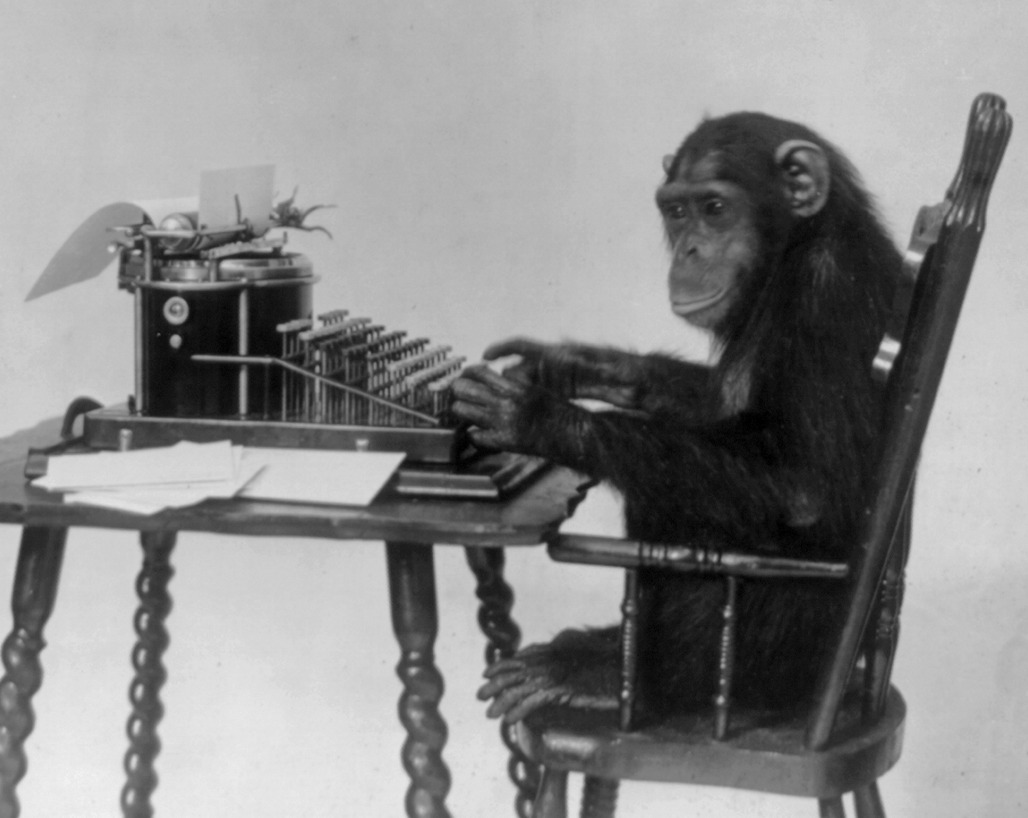
\includegraphics[width=0.3\textwidth]{figures/chimpanzee.jpg}
\end{center}
\end{example}
\newpage 

\subsubsection{Kolmogorov's 0-1 Law}
We look at a generalisation of the Borel-Cantelli Lemma. To begin, let us define the notion of tail events and tail $\sigma$-algebra by first introducing some notations:
\begin{definition}
Let $(\Omega, \F, \p)$ be a probability space: 
\begin{enumerate}
    \item Let $\F_1, \F_2, ...$ be sub-$\sigma$-algebra of $\F$. Define the $\sigma$-algebra generated by their union:
    \begin{equation}
        \bigvee_{i=1}^n \F_i = \sigma\bracket{\bigcup_{i=1}^n \F_i},
    \end{equation}
    and extend this definition to the case when $n=\infty$.
    \item Let $\xi_1, \xi_2,...$ be a sequence of random variables defined on this probability space. Then
    \begin{equation}
        \sigma(\xi_1,\xi_2,...,\xi_n) = \bigvee_{i=1}^n \sigma(\xi_i),
    \end{equation}
    with this definition being extended to the infinite case.
\end{enumerate}
\end{definition}

\begin{definition}
Under the above settings, define $\F_n^p = \sigma (\xi_n, \dots, \xi_p)$ for $p\geq n$ and $\F_n^\infty = \sigma (\xi_n, \dots)$ (representing the future information), then the $\sigma-$ algebra associated with the sequence of random variables $\xi_1, \xi_2, ...$ is
\begin{equation*}
    \cT = \bigcap_{n=1}^\infty \F_n^\infty
\end{equation*}
is called the \textbf{tail $\sigma-$algebra}. Events of $\cT$ are called tail events.
\end{definition}

We are more interested in studying tail $\sigma$-algebra associated with a mutually independent sequence of random variables $\xi_1, \xi_2, ...$. If this assumption holds, then we have the following observation:
\begin{lemma}
For all $n \geq 2$, $\F_1^n$ and $\F_{n+1}^\infty$ are independent.
\end{lemma}

\begin{proof}
Recall the shortcut developed in lemma \ref{lem:independence_shortcut}! We first prove that $\F_1^n$ is independent with $\F_{n+1}^p$ for any $n+1 \leq p < \infty$. Note that $\F_1^n$ is generated by the $\pi$-system $\cup_{i=1}^n \sigma(\xi_i)$ and $\F_{n+1}^p$ is similarly generated by the $\pi$-system $\cup_{i=n+1}^p \sigma(\xi_i)$, and that these $\pi$-systems are independent, so we know that $\F_1^n$ is independent with $\F_{n+1}^p$ for any finite $p$. Now note that $\F_n^\infty$ is generated by the $\pi$-system $\cup_{p\geq n+1} \F_{n+1}^p$, so $\F_1^n$ is generated by $\F_{n+1}^\infty$.
\end{proof}

Note that $\cT \subseteq \F_n^\infty$ for any \textbf{finite} $n \geq 1$, so we have $\cT$ being independent with any $\F_1^n$. This provides an interpretation of the definition of a tail event $A \in \cT$, that \textit{its occurrence is independent of a finite number of changes in values of $\xi_n$}. An important example will be to note that the convergence of a sequence of random variable $\xi_1, \xi_2, ...$ is not affected when only a finite number of $\xi_n$'s are changed. 

\begin{example}
We see, for example, that $\set{\xi_{10} \in B}$ may not be in $\cT$, since its occurrence may be affected by changing a finite number of $\xi_n$, in our case being $\xi_{10}$. We also note that $\set{\omega \,|\, \forall n, \, \xi_n \notin \B}$ is not in $\cT$ since its occurrence may change by just affecting a value of $\xi_n$.
\end{example}

In fact, the above observations lead to a more surprising result! Since $\cup_{n\geq 1} \F_1^n$ is a $\pi$-system generating $\F_1^\infty$, we see that $\cT$ is independent with $\F_1^\infty$, and hence $\cT$ is actually independent with itself! This leads to the well-known Kolmogorov's Zero-One Law.

\begin{theorem}[Kolmogorov's Zero-One Law]
Let $\xi_1, \xi_2, \dots$ be a sequence of independent random variables, and let $A \in \cT$. Then $\p(A)$ can only have a value of zero or one.
\end{theorem}

\begin{proof}
We have $\p(A) = \p(A \cap A) = (\p(A))^2$, so $\p(A)$ must has value zero or one. 
\end{proof}

\begin{example}
Given independent sequence $\xi_1, \xi_2, ...$ and $B_1, B_2, ... \in \B(\R)$, then $\set{\xi_n \in B_n \text{ i.o.}} = \cap_{n=1}^\infty \cup_{k\geq n} \set{\xi_k \in B_k} \in \cT$. Now consider the independent events $A_1, A_2, ...$, then the sequence of random variables $\chi_{A_1}, \chi_{A_2}, ...$ are independent, and that the event $\limsup_{n} A_n := \set{\chi_{A_i} = 1 \text{ i.o.}}$ is a tail event associated with this independent sequence of random variables. The Kolmogorov's Zero-One Law then says that $\limsup_{n} A_n$ must have probability zero and one, which coincides with our observation from the Borel-Cantelli lemmas.
\end{example}

Perhaps the most important application of Kolmogorov's Zero-One Law is that it says that a random series of \textbf{independent} random variables must converge or diverge almost surely. Let $\xi_1, \xi_2, ...$ be sequence of independent random variables. Then obviously the following function is $\F_k^\infty$ measurable:
\begin{equation*}
    \limsup_{n\to\infty} \sum_{i\geq k} \xi_i, \quad \liminf_{n\to\infty} \sum_{i\geq k} \xi_i, \quad \lim_{n\to\infty} \sum_{i\geq k} \xi_i
\end{equation*}

As a result, the following functions are $\cT$ measurable:
\begin{equation*}
    \limsup_{n\to\infty} \sum_{i\geq 1} \xi_i, \quad \liminf_{n\to\infty} \sum_{i\geq 1} \xi_i, \quad \lim_{n\to\infty} \sum_{i\geq 1} \xi_i
\end{equation*}

In particular, the following set is a tail event associated with the given independent sequence of random variables:
\begin{equation*}
A = \set{\omega \, \bigg| \, \sum_{i\geq 1} \xi_i \text{ exists}},
\end{equation*}

and as a result of the Kolmogorov 0-1 law, we have the following 
\begin{corollary}
If $\xi_1, \xi_2, \dots$ is a sequence of independent random variables, then $\sum_{n=1}^\infty \xi_n$ either converges a.s. or diverges a.s.
\end{corollary}

We finally note an application of Kolmogorov 0-1 law:
\begin{example}
Let $\eta$ be a real-valued random variable that is measurable with respect to the $\sigma-$algebra $\cT$, i.e. $\{ \eta \in B\} \in \cT,$ $B \in \B(\R)$. Then $\eta$ is degenerate, i.e. there is a constant $c$ such that $\p(\eta = c) = 1$.
\end{example}

\begin{proof}
Note that for all $x \in \R$ one have $\p(\eta \leq x) \in \set{0,1}$ by the Kolmogorov 0-1 law. Take $c = \inf_{x \in \R \,|\, \p(\eta \leq x) = 1}$. Such an infinmum exists given that the distribution function is increasing, so if the infinmum does not exists then it means $0 = \p(\varnothing) = \p(\eta \leq -\infty) = 1$, which is a contradiction. It is easy to check that $\p(\eta = c) = 1$ by utilising the fact that $\p(\eta \leq x)$ is an increasing cadalag, and we will leave it as an exercise.
\end{proof}

There are many more zero-one laws in probability theory, but we will defer the discussion of those statements to a later chapter.
\newpage 

\subsection{More on Almost Sure Convergence}
\subsubsection{Almost sure convergence implies convergence in probability}
Recall the definition of almost sure convergence: a sequence $\xi_1, \xi_2, \dots$ of random variables converges almost surely to the random variable $\xi$ (denoted as $\xi_n \xrightarrow{a.s} \xi$) if $\p(\set{\omega \,|\, \xi_n(\omega) \not \to \xi(\omega)}) = 0$. This section is dedicated to explore the relationships between almost sure convergence, $L^p$ convergence and convergence in probability. As a warm up, we begin by the following equivalent definition of almost sure convergence.

\begin{proposition} \label{prop:as_prob_conv}
A necessary and sufficient condition that $\xi_n \to \xi$ $\p$-almost surely is that 
\begin{equation*}
    \p \bigg(\sup_{k \ge n} |\xi_k - \xi| \ge \varepsilon\bigg) \to 0, \quad n \to \infty,
\end{equation*}
    for every $\varepsilon > 0$.
\end{proposition}

\begin{hint}
The key step is to rewrite the set $\set{\xi_n \not\to \xi}$ into a countable union of sets. From the definition of convergence, we have
$$\xi_n(\omega) \not\to \xi(\omega) \iff \exists \, \epsilon > 0 \text{ s.t. } |\xi_n(\omega) - \xi(\omega)| \geq \epsilon \text{ infinitely often.}$$
So if we let $A_n^\varepsilon= \{ \omega: |\xi_n - \xi| \ge \varepsilon\}$ and $A^\varepsilon= \limsup A_n^\varepsilon= \{A_n^\varepsilon\, \text{ i.o.} \}$, then we have 
$$\{\omega \,|\, \xi_n(\omega) \not \to \xi(\omega) \} = \bigcup_{\varepsilon \ge 0} A^\varepsilon.$$
But this is not a countable union. Fortunately, the sets $A^\epsilon$ are nested, so one can restrict $\epsilon$ to the form $\epsilon = 1/m$ for some positive integers $m$, so we have
\begin{equation*}
\{\omega \,|\, \xi_n(\omega) \not \to \xi(\omega) \} =  \bigcup_{m=1}^\infty A^{1/m}.
\end{equation*}
The remaining of proof utilises the fact that the sets $A^\epsilon$ are nested.
\end{hint}

\begin{proof}
By nestedness of $A^\epsilon$ we have the following chain of implications:
\begin{align*}
    \p(\set{\omega: \xi_n \not \to \xi}) = 0 
    &\iff \p \bigg( \bigcup_{\varepsilon > 0} A^\varepsilon \bigg) = 0\\
    &\iff \p \bigg( \bigcup_{m=1}^\infty A^{1/m} \bigg) = 0\\
    &\overset{(*)}{\iff} \forall m \geq 1, \; \p(A^{1/m}) = 0\\
    &\iff \forall \varepsilon > 0, \; \p(A^\varepsilon) = 0
\end{align*}
The equivalence $(*)$ is justified below: first note that $\p(A^{1/m}) \leq \p(\cup_{m\geq 1} A^{1/m})$ so ($\Rightarrow$) clearly follows. The ($\Leftarrow$) direction follows from union bound: $\p(\cup_{m\geq 1} A^{1/m}) \leq \sum_{m\geq 1} \p(A^{1/m}) = 0$.\\

To complete the proof, we note that
\begin{equation*}
    \p(A^\varepsilon) = \p \bigg( \bigcap_{n \geq 1} \bigcup_{k \ge n} A_k^\varepsilon \bigg) = \lim_n \p \bigg( \bigcup_{k \ge n} A_k^\varepsilon \bigg) = \p\bigg(\sup_{k \ge n}|\xi_k - \xi| \ge \varepsilon \bigg),
\end{equation*}
so the result follows.
\end{proof}

From this equivalent statement, it is clear that almost sure convergence implies convergence in measure. In our summary diagram, we have proven the following highlighted implication.

\begin{figure} [H]
    \centering
    \begin{tikzcd}
    & \overset{L^p}{\to} \arrow[Rightarrow, d]  & \\
    \textcolor{red}{\overset{a.e.}{\to}} \arrow[Rightarrow, r, red] & \textcolor{red}{\overset{p}{\to} \arrow[Rightarrow, r]} & \overset{d}{\to}
\end{tikzcd}
\end{figure}

\begin{exercise}[Cauchy-like condition for almost sure convergence] \label{ex:as_Cauchy}
Show that the sequence $\{\xi_n\}_{n\geq 1}$ converges almost surely iff, for all $\varepsilon > 0$, 
\begin{equation*}
    \lim_{n\to\infty} \p \bigg(\sup_{k, l \ge n} |\xi_{k} - \xi_l| \ge \varepsilon\bigg) = 0,
\end{equation*}
or equivalently,
\begin{equation*}
    \p \bigg(\sup_{k \ge 0} |\xi_{n+k} - \xi_n| \ge \varepsilon\bigg) \to 0, \quad n \to \infty.
\end{equation*}
\end{exercise}

\begin{hint}
Let
\begin{equation*}
    B_{k,l}^\varepsilon = \{ \omega: |\xi_k - \xi_l| \ge \varepsilon\} , \quad B^\varepsilon = \bigcap_{n=1}^\infty \bigcup_{k, l \ge n} B_{k,l}^\varepsilon.
\end{equation*}
Then 
$$\{ \omega: \{\xi_n(\omega) \}_{n\ge1} \text{ is not convergent} \} = \bigcup_{\varepsilon > 0}B^\varepsilon,$$ 
and it can be shown as in proposition \ref{prop:as_prob_conv} that 
$$\p(\{ \omega: \{\xi_n(\omega) \}_{n\ge1} \text{ is not convergent} \}) = 0$$ 
if and only if the statement in the theorem holds.
\end{hint}

\subsubsection{Convergence in probability does not imply almost sure convergence}

The following counter-examples demonstrate that both convergences in probability and convergences in $L^p$ do not imply almost convergence. 

\begin{example}
Let $\xi_1, \dots, \xi_n$ be independent random variables on a certain probability space $(\Omega,\F,\p)$ taking value from $\set{0,1}$ with
\begin{equation*}
    \p(\xi_n = 1) = 1/n, \quad \p(\xi_n = 0) = 1 - 1/n.
\end{equation*}
We may choose $(\Omega,\F) = (\set{0,1}, \B(\set{0,1}))^{\N}$ and $\p$ being an appropriate infinite product measure. Then
\begin{equation*}
    \E[|\xi_n - 0|^p] = 1/n \to 0, \text{ so } \xi_n \xrightarrow{L^p} 0.
\end{equation*}
However, 
\begin{equation*}
    \{ \omega: \xi_n \to 0 \} = \{ \xi_n = 0 \text{ everywhere} \} = \bigcup_{n=1}^\infty \underbrace{\bigcap_{k \ge n} \{ \xi_k = 0 \}}_{\text{increasing sequence of sets}}
\end{equation*}
Therefore, 
\begin{align*}
    \p(\xi_n \to 0) &= \lim_{n \to \infty} \p \bigg(\bigcap_{k\ge n} \{ \xi_k = 0\} \bigg)\\
    &= \lim_{n \to \infty} \prod_{k \ge n} \p(\xi_k = 0)\\
    &= \lim_{n \to \infty} \prod_{k \ge n} \bigg(1 - \frac{1}{k}\bigg) = 0
\end{align*}
Indeed,
\begin{equation*}
    \prod_{k \ge n} \bigg( 1- \frac{1}{k} \bigg) = \lim_{N \to \infty} \prod_{k=n}^N \frac{k-1}{k} = \lim_{N \to \infty} \frac{n-1}{n} \frac{n}{n+1} \cdots \frac{N-1}{N} = 0.
\end{equation*}
Thus $\xi_n \not \xrightarrow{a.s.} 0$.
\end{example}

\begin{example}[Typewriter Sequence]
We provide another example on $([0,1], \B([0,1]), \Leb)$ with a similar flavor as the previous example. Consider the sequence 
\begin{equation}
f_n := \chi_{A_n}, \quad A_n = \sqbracket{\frac{n}{2^k} - 1, \frac{n+1}{2^k} - 1}
\end{equation}
whenever $k \geq 0$ and $2^k \leq n < 2^{k+1}$ The first few $A_n$ is as followed: 
$$[0,1], [0,1/2], [1/2, 1], [0,1/4], [1/4,1/2], [1/2,3/4], [3/4,1], ...$$
You can plot the indicator functions yourself, or look at some demonstrations on websites. \footnote{e.g. \url{https://math.stackexchange.com/questions/1412091/the-typewriter-sequence}}. You will see that the indicator functions move from left to right over $[0,1]$, then half its width and repeat again, which provides an explanation of the sequence's name. \footnote{Figure provided by Dr. Shordzi under the Creative Common 2.0 License: \url{https://creativecommons.org/licenses/by-sa/2.0/}}

\begin{center}

\includegraphics[width=0.4\textwidth]{figures/typewriter.jpg}
\end{center}

The convergence in $L^p$ for any $p < \infty$ (hence convergence in $L^p$) of the sequence to zero is proven by noting that the width of indicator function vanishes as $n \to \infty$. However, given that the indicator function moves from left to right infinitely many times, for all $\omega \in [0,1]$, $f_n(\omega) = 1$ (and 0) infinitely often. As a result, $f_n(\omega)$ does not converge almost surely.
\end{example}

However, the implication from almost sure convergence to convergence in probability admits a partial converse: if a sequence converges in probability, then we can extract a subsequence that converges almost surely. To prove this important result, we note that 

\begin{lemma} \label{lem:as_conv_sufficient}
A sufficient condition for $\xi_n \xrightarrow{a.s.} \xi$ is that
\begin{equation*}
    \sum_{n=1}^\infty \p(|\xi_n - \xi| \ge \varepsilon) < \infty 
\end{equation*}
is satisfied for all $\varepsilon > 0$.
\end{lemma}

\begin{proof}
Denote the event $A_n^\varepsilon = \{\omega \,|\, |\xi_n(\omega) - \xi(\omega)| \ge \varepsilon\}$ as required. Since $\sum_{k\geq 1} \p(A^\epsilon) < \infty$, by first Borel-Cantelli lemma we know that $\p(A^\varepsilon) := \p(A_n^\epsilon \; \text{i.o.}) = 0$. Following the arguments in proposition \ref{prop:as_prob_conv} we know that $\p(\set{\omega \,|\,\ \xi_n \not\to \xi}) = 0$ as desired.
\end{proof}

\begin{corollary} \label{cor:as_conv_sum_sufficient}
Let $(\varepsilon_n)_{n\ge 1}$ be a sequence of positive numbers such that $\varepsilon_n \downarrow 0$ as $n \to \infty$. Then if $\xi_n$ converges to $\xi$ in probability sufficiently fast in the sense that 
\begin{equation*}
    \sum_{n=1}^\infty \p(|\xi_n - \xi| \ge \varepsilon_n) < \infty,
\end{equation*}
then $\xi_n \xrightarrow{a.s.} \xi$.
\end{corollary}

\begin{proof}
Fix an arbitrary $\epsilon > 0$. Choose $N$ such that for all $n \geq N$ we have $\epsilon_n < \epsilon$. Then 
\begin{equation*}
    \sum_{n=1}^\infty \p(|\xi_n - \xi| \geq \epsilon) \leq \underbrace{\sum_{n=1}^{N-1} \p(|\xi_n - \xi| \geq \epsilon)}_{\leq N-1 < \infty} + \underbrace{\sum_{n=N}^\infty \p(|\xi_n - \xi| \geq \epsilon)}_{<\infty},
\end{equation*}
hence by the above lemma \ref{lem:as_conv_sufficient} we have $\xi_n \overset{\text{a.s.}}{\to} \xi$ as $n \to \infty$.
\end{proof}

We may now prove our key result for this subsection.
\begin{theorem} \label{thm:subsequence_conv_prob}
If $\xi_n \xrightarrow{p} \xi$, then there exists a subsequence such that
\begin{equation*}
    \xi_{n_k}\xrightarrow{a.s.} \xi.
\end{equation*}
\end{theorem}

\begin{proof}
Since $\lim_{n \to \infty} \p(|\xi_n - \xi| > 1/k) = 0$ for all $k \ge 1$, we can choose a subsequence such that 
\begin{equation*}
    \p (|\xi_n - \xi| > k^{-1}) \le 2^{-k} \quad \forall k \ge 1
\end{equation*}
Since $\sum_{k=1}^\infty 2^{-k}$ converges, by above corollary \ref{cor:as_conv_sum_sufficient} we have $\xi_{n_k}\xrightarrow{a.s.} \xi$.
\end{proof}

The trick of extracting a almost surely convergent subsequence is very helpful in justifying limits. Here is an immediate application of the above theorem:
\begin{corollary}
If $\xi_1 \ge \xi_2 \ge \cdots \ge 0$, are random variables and $\xi_n \xrightarrow{p} 0$, then
\begin{equation*}
    \xi_n \xrightarrow{a.s.} 0.
\end{equation*}
\end{corollary}

\begin{proof}
Note that $\xi_n \xrightarrow{a.s} 0 $ if and only if $\limsup \xi_n = 0$ a.s. Let $\varepsilon > 0$. Denote $A_n = \{\xi_n > \varepsilon \}$. Then by continuity,
\begin{equation*}
    \p(\limsup \xi_n > \varepsilon) = \p(\xi_n > \varepsilon \, i.o.) = \lim_{n \to \infty} \p\bigg(\bigcup_{k \ge n} A_k\bigg).
\end{equation*}
Since $A_n$ is non-increasing, the right hand side equals $\lim_{n \to \infty} \p(A_n)$ which is $0$ since $\xi_n \xrightarrow{p} 0$. Thus 
\begin{equation*}
    \p(\limsup \xi_n > \varepsilon) = 0 \quad \forall \varepsilon > 0,
\end{equation*}
and therefore
\begin{equation*}
    \p(\xi_n \not \to \xi) \le \sum_{m=1}^\infty \p(\limsup \xi_n > 1/m) = 0.
\end{equation*}
\end{proof}

\begin{unexaminable}
We finally note an observation regarding convergence in probability:
\begin{corollary}
Let $\xi, (\xi_n)_{n\geq 1}$ be random variables on the probability space $(\Omega,\F,\p)$. Then $\xi_n \to \xi$ in probability as $n \to \infty$ iff for any subsequence, ther is a further subsequence that converges $\p$-a.s. to $\xi$.
\end{corollary}
\begin{proof}
The $(\Rightarrow)$ direction is proven in theorem \ref{thm:subsequence_conv_prob}. For $(\Leftarrow)$, we note that almost sure convergence implies convergence in probability. We also recall a basic fact that in metric space, if $(a_m)$ is a sequence such that for any subsequence there is a further subsequence that converges to some element $a$, then $a_m \to a$. Since convergence in probability is metrisable as shown in exercise \ref{ex:metric_for_conv_in_prob}, we may directly use this result to complete the proof.
\end{proof}
\end{unexaminable}

\begin{exercise}
\begin{enumerate}
    \item[]
    \item Let $\xi_1, \xi_2, \dots, \xi_n$ be i.i.d. random variables with the standard exponential distribution and define
    \begin{equation*}
        M_n = \max \{\xi_1, \dots, \xi_n \}.
    \end{equation*}
    Show that as $n \to \infty$
    \begin{itemize}
        \item $\limsup \xi_n/\log{n} = 1$ a.s.
        \item $M_n / \log{n} = 1$ a.s.
    \end{itemize}
\end{enumerate}
\end{exercise}

\subsubsection{Almost sure convergence and $L^p$ convergence}
It has been proven in elementary measure theory classes that having almost sure convergence does not guarantee $L^p$ convergence. Here we prove a result which states that if we have almost sure convergence and convergence in mean, then we have $L^1$ convergence.
\begin{theorem}
Let $\xi_n$ be a sequence of nonnegative random variables such that $\xi_n \xrightarrow{a.s.} \xi$ and $\E[\xi_n] \to \E[\xi] < \infty$. Then $\xi_n \xrightarrow{L^1} \xi$, or 
\begin{equation*}
    \E[|\xi_n - \xi|] \to 0, \quad n\to \infty.
\end{equation*}
\end{theorem}

\begin{proof}
We have $\E[|\xi_n|] < \infty$ for sufficiently large $n$ and therefore for such $n$ we have
\begin{align*}
    \E[|\xi_n - \xi|] &= \E[\xi - \xi_n]\chi_{\xi \ge \xi_n} + \E[\xi_n - \xi]\chi_{\xi_n \ge \xi}\\
    &= 2 \E[\xi - \xi_n]\chi_{\xi \ge \xi_n} + \E[\xi_n - \xi].
\end{align*}
But $0 \le (\xi - \xi_n) \chi_{\xi \ge \xi_n} \le \xi$. Therefore, by the dominated convergence theorem, $\E[\xi-\xi_n] \chi_{\xi \ge \xi_n} \to 0$.
\end{proof}

\subsection{Strong Law of Large Numbers}
We are now ready to prove some strong law of large numbers. A strong law of large number is the statement of the following form: given $\xi_1, \xi_2, \dots$ is a sequence of integrable random variables, which is assumed to be independent (or "weakly correlated"). Let $S_n = \xi_1 + \xi_2 + ... + \xi_n$, then the sequence $(\xi_n)_{n\geq 1}$ is said to satisfy the strong law of large numbers if 
\begin{equation*}
    \frac{S_n - \E[S_n]}{n} \xrightarrow{\text{a.s.}} 0.
\end{equation*}
It is stronger than the weak law of large number as proven in chapter 4 in the sense that we only have convergence in probability in contrast to almost sure convergence. \\

Recall that for i.i.d. $\xi_n$ with a second moment assumption (i.e. $\V[\xi_1] < \infty$) we have the $L^2$ weak law of large number. If we impose an excessive moment assumptions, we can prove a strong law of large number.

\begin{proposition}[Cantelli's Strong Law of Large Numbers]
Let $\xi_1, \xi_2, \dots$ be i.i.d. random variables with $\E[\xi_1^4] < \infty$. Then
\begin{equation}
    \frac{S_n - \E[S_n]}{n} \xrightarrow{\text{a.s.}} 0,
\end{equation}
i.e. $\{ \xi_n \}$ satisfies the strong law of large numbers.
\end{proposition}

\begin{hint}
Without loss of generality we centralise the random variables by substracting its mean, then $\E[\xi_1] = \E[\xi_1^3] = 0$. Fix an arbitrary $\epsilon > 0$, we hope to use lemma \ref{lem:as_conv_sufficient} to establish almost sure convergence. We will bound the probability $\p(|S_n/n| \geq \epsilon) = \p(|S_n| \geq n\epsilon)$ by using Chebyshev inequality.
\end{hint}

\begin{proof}
Let us therefore bound the probability $\p(|S_n/n| \geq \epsilon)$, so that it decays fast enough and $\sum_{n\geq 1} \p(|S_n/n|\geq \epsilon) < \infty$. We might therefore want $\p(|S_n|\geq n\epsilon) = O(1/n^2)$. \\

To use the Chebyshev inequality, one has to bound the $k$-th moment of $S_n/n$ (where $k$ is an even number). We want the $k$-th moment to be of order $O(1/n^2)$. We may look at second moments:
\begin{equation}
\V[S_n/n] = n\E[\xi_1]/n^2,
\end{equation}
which is not enough for Chebyshev inequality. We have to look at the forth moments. In the expansion of forth moments, the only non-vanishing terms are terms of the form $\E[\xi_j^4]$ and $\E[\xi_i^2 \xi_j^2] = \E[\xi_i^2] \E[\xi_j^2]$ with $i \neq j$, noticing that the odd moments of $\xi_i$ vanishes. We therefore have the expansion
\begin{equation}
\E[S_n^4] = \E\sqbracket{\sum_{k=1}^n \xi_k^4 + {4 \choose 2, 2} \sum_{j,k=1, j < k} \xi_j^2 \xi_k^2}
\end{equation}
where ${4 \choose 2,2} = 4!/(2!)^2 = 6$ comes from the multinomial theorem. Now notice that there are $n(n-1)/2$ unique ways to choose the indices $(j,k)$ such that $j < k$, therefore we have, from the i.i.d. assumption,
\begin{equation}
\E[|S_n/n|^4] = \frac{1}{n^4} \bracket{n\E[\xi_1^4] + 3n(n-1) (\E[\xi_1^2])^2}
\end{equation}
Finally, note from Lyapunov inequality (corollary \ref{cor:lyapunov_ineq}) that $\E[\xi_1^2]^{1/2} \leq \E[\xi_1^4]^{1/4}$, so we have 
\begin{equation}
\E[|S_n/n|^4] \leq \frac{3n^2 - 2n}{n^4}\E[\xi_1^4] \lesssim \frac{1}{n^2},
\end{equation}
and therefore $\sum_{n\geq 1} \p(|S_n/n|\geq \epsilon) \lesssim \sum_{n\geq 1} n^{-2} < \infty$ as desired.
\end{proof}

This strong law of large number is already very useful for practical purposes. It can be used when $\xi_1$ follows common distributions (e.g. Normal, Gamma, Binomial, ...), or have finite supports. However, as seen below, we can impose much weaker assumptions on the moments of $\xi_i$. \\

We will follow Kolmogorov's approaches in proving his strong law of large numbers. The approach is cumbersome since it involves many technical lemma in analysis, nevertheless it opens up routes of proving more general statements about convergence of random series. Another route is to consider truncation of random variables, which is simpler and actually leads to a stronger version of strong law of large number by Etemadi as proved in \cite{EtemadiSLLN}. We will not cover this proof in our notes. \\

Back to Kolmogorov's approach. Let us start with the following Kolmogorov maximal inequality:

\begin{proposition}[Kolmogorov's maximal inequality]
Let $\xi_1, \xi_2, \dots$ be independent random variables with finite variances. Then $\forall n \ge 1$ and $x > 0$, we have 
\begin{equation*}
    \p\bracket{\max_{1 \le k \le n} | S_k - \E[S_k]| \ge x} \le \frac{\V[S_n]}{x^2}.
\end{equation*}
\end{proposition}

Notice that this is a stronger version of the Chebyshev inequality, since Chebyshev inequality only gives
\begin{equation*}
    \p\bracket{|S_k - \E[S_k]| \geq x} \leq \frac{\V[S_n]}{x^2}.
\end{equation*}

Combining with union bound we get
\begin{equation*}
    \p\bracket{\max_{1\leq k \leq n} |S_k - \E[S_k]| \geq x} = \p\bracket{\bigcup_{k=1}^n \set{|S_k - \E[S_k]| \geq x}} \leq \frac{\textcolor{blue}{n}\V[S_n]}{x^2}.
\end{equation*}

What this maximal inequality does is to remove the factor of $n$ generated in the union bound. As seen in \ref{lem:as_conv_sufficient}, if we are able to bound the probability of maximum deviation using maximal inequalities, then we can use Borel-Cantelli to establish almost sure convergence.

\begin{hint}
Again we subtract the random variables with its mean to set $\E[\xi_1] = 0$. The key step is to note that the events $A_k, k=1,...,n$ is a partition of $A = \set{\omega\,|\, \max_{1\leq k \leq n} |S_k(\omega)| \geq x}$, where $|S_j|$ first exceeds $x$ at $j=k$, i.e.
\begin{equation*}
    A_k := \set{\omega \,|\, |S_j(\omega)| < x \text{ and } |S_k(\omega)| \geq x}.
\end{equation*}
Now show that $\E[S_n^2 \chi_{A_k}] \geq x^2 \p(A_k)$ by breaking up $S_n$.
\end{hint}

\begin{proof}
From the above hint, we have
\begin{equation*}
    \V[S_n^2] \geq \E[S_n^2 \chi_A] = \sum_{k=1}^n \E[S_n^2 \chi_{A_k}].
\end{equation*}
But 
\begin{align*}
    \E[S_n^2 \chi_{A_k}] &= \E[(S_k + \xi_{k+1} + ... + \xi_n)^2 \chi_{A_k}] \\
    &= \underbrace{\E[S_k^2 \chi_{A_k}]}_{\geq x^2 \p(A_k)} + \underbrace{2\E[(S_k \chi_{A_k})(\xi_{k+1} + ... + \xi_n)]}_{= 2\E[S_k \chi_{A_k}] \E[\xi_{k+1} + ... + \xi_n] = 0} + \underbrace{\E[(\xi_{k+1} + ... + \xi_n)^2]}_{\geq 0} \\
    &\geq x^2 \p(A_k),
\end{align*}
so we have
\begin{equation}
    \V[S_n^2] \geq x^2 \sum_{k=1}^n \p(A_k) = x^2 \p(A).
\end{equation}
\end{proof}

With this maximal inequality, we may prove the Kolmogorov's three series theorem, which states that the almost sure convergence of a (truncated) random series depends on the convergence of three deterministic series. Here we will prove the statement in three steps:

\begin{lemma}[Three series theorem, part I]
Suppose $\xi_1, \xi_2, ...$ are independent real-valued series and have $\E[\xi_i] = 0$ for all $i$. If we know that $\sum_{i\geq 1} \V[\xi_i] < \infty$, then $\sum_{i\geq 1} \xi_i$ converges almost surely.
\end{lemma}

\begin{proof}
Since we are not given the limit for which the random series converges, the best way of proving this theorem is to resort on proving the series $S_n := \sum_{i=1}^n \xi_i$ being Cauchy as in exercise \ref{ex:as_Cauchy}. To this we need to show that as $n \to \infty$,
\begin{equation*}
    \p\bracket{\sup_{k\geq 1} |S_{n+k} - S_k| \geq \epsilon} \to 0
\end{equation*}
We note that for all $m < \infty$ we have, from the above maximal inequality,
\begin{equation}
    \p\bracket{\sup_{1 \leq k \leq m} |S_{n+k} - S_k| \geq \epsilon} \leq \epsilon^{-2} \sum_{k=1}^m \V[\xi_{n+k}] \leq \epsilon^{-2} \sum_{k=1}^\infty \V[\xi_{n+k}],
\end{equation}
so one can send $m \to \infty$ (by continuity from below):
\begin{equation}
\p\bracket{\sup_{k \geq 1} |S_{n+k} - S_k| \geq \epsilon} \leq \sum_{k=1}^\infty \V[\xi_{n+k}] \overset{n \to \infty}{\to} 0
\end{equation}
as desired, so the series $S_n$ converges almost surely.
\end{proof}

\begin{theorem}[Three series theorem, part II]
Let $\xi_1, \xi_2, \dots$ be independent random variables. If $\sum_{n=1}^\infty \E[\xi_n]$ and $\sum_{n=1}^\infty \V[\xi_n]$ converge, then $\sum_{n=1}^\infty \xi_n$ converges a.s.
\end{theorem}

\begin{proof}
This follows by breaking the random series into two parts:
\begin{equation}
\sum_{i=1}^\infty \xi_i = \sum_{i=1}^\infty (\xi_i - \E[\xi_i]) + \sum_{i=1}^\infty \E[\xi_i],
\end{equation}
provided that the two series in the RHS actually converges, so the theorem follows.
\end{proof}

\begin{unexaminable}
The above three series theorem is enough for our application, but for completion let us state the full Kolmogorov's three series theorem:
\begin{corollary}[Three series theorem, part III] 
Let $\xi_1, \xi_2, ...$ be independent random variables. Let further $A>0$, and $\eta_i = \xi_i \chi_{|\xi_i| \leq A}$ be the truncated random variables. Then $\sum_{i\geq 1} \xi_i$ converges almost surely if and only if the following three series converges:
\begin{center}
(1) $\sum_{i\geq 1} \p(|\xi_i| > A)$, (2) $\sum_{i\geq 1} \E[\eta_i]$ and (3) $\sum_{i\geq 1} \V[\eta_i]$
\end{center}
When $A = \infty$ this theorem reduces to part II.
\end{corollary}

\begin{proof}
We only prove the sufficiency part. Notice that part II guarantees that $\sum_{i\geq 1} \eta_i$ converges almost surely, and the convergence of $\sum_{i\geq 1} \p(|\xi_i| > A)$ means that $\p(|\xi_i| > A \text{ i.o.}) = 0$ by the first Borel-Cantelli lemma. Therefore, almost surely $\xi_i = \eta_i$ eventually, and in such case $\sum_{i\geq 1} \xi_i$ converges.
\end{proof}
\end{unexaminable}

We are half-way through proving Kolmogorov's strong law of large number. To complete the proof we have to prove a few technical lemmas concerning the convergence of weighted mean of the first terms of a converging sequence. You should be able to prove the following lemmas yourself using tools from elementary analysis classes.

\begin{lemma}[Toeplitz] \label{lem:Toeplitz}
Let $\{a_n\}$ be a sequence of nonnegative numbers, $b_n = \sum_{i=1}^n a_i$, $b_1 = a_1 > 0$, and $b_n \uparrow \infty, n \to \infty$. Let $\{ x_n \}_{n \ge 1}$ be a sequence of numbers converging to $x$. Then
\begin{equation*}
    \frac{1}{b_n} \sum_{j=1}^n a_j x_j \to x.
\end{equation*}
In particular, if $a_n = 1$, then
\begin{equation*}
    \frac{x_1 + \cdots + x_n}{n} \to x.
\end{equation*}
\end{lemma}

\begin{hint}
Observe that for all $1 \leq N \leq n$,
\begin{equation*}
\abs{\frac{1}{b_n}\sum_{j=1}^n a_j x_j - x} = \abs{\frac{1}{b_n}\sum_{j=1}^n a_j(x_j - x)} \leq \abs{\frac{1}{b_n}\sum_{j=1}^N a_j(x_j - x)} + \abs{\frac{1}{b_n}\sum_{j=N+1}^n a_j(x_j - x).}
\end{equation*}
Now choose $N$ such that $|x_j - x|$ is sufficiently small. Show that the tail (second term of RHS) is very small. Can you complete the proof from here?
\end{hint}

\begin{proof}
Fix $\epsilon > 0$. Choose $N_0 := N_0(\epsilon)$ such that for all $n \geq N_0$ we have $|x_j - x| < \epsilon/2$. Now choose $N_1 > N_0$ (which depends on $N_0$) such that $b_{N_1}^{-1} \sum_{j=1}^{N_0} |x_j - x| < \epsilon/2$, which exists since $|x_j - x|$ is bounded for $j = 1,...,N_0$. Then for any $n > N_1$, we have
\begin{align*}
\abs{\frac{1}{b_n}\sum_{j=1}^n a_j x_j - x} &\leq \abs{\frac{1}{b_n}\sum_{j=1}^{N_0} a_j(x_j - x)} + \abs{\frac{1}{b_n}\sum_{j=N+1}^n a_j(x_j - x)} \\
&\leq \frac{1}{b_{N_1}} \abs{\sum_{j=1}^N a_j(x_j - x)} + \abs{\frac{1}{b_n}\sum_{j={N_0}+1}^n a_j(x_j - x)}\\
&< \frac{\epsilon}{2} + \frac{\epsilon}{2} \underbrace{\bracket{\frac{1}{b_n} \sum_{j=N_0+1}^n a_j}}_{\leq 1} \leq \epsilon,
\end{align*}
so we have the above convergence.
\end{proof}

Here we give an application of the Toeplitz lemma by the following exercise:
\begin{exercise}
Suppose $(\xi_i)_{i\geq 1}$ is a sequence of independent random variables with common mean $m$ and variance $\V[\xi_k] = k\eta(k)$ with the condition that $\V[\xi_k] \to \infty$, but $\eta(k) > 0$ and $\eta(k) \searrow 0$ as $k \to \infty$. Use Toeplitz lemma to prove that the sequence satisfies weak law of large number, that $n^{-1} \sum_{i=1}^n \xi_i \to m$ as $n \to \infty$ in $L^2$ and in probability.
\end{exercise}

We then prove the Kronecker lemma.
\begin{lemma}[Kronecker]
Let $b_n$ be a sequence of positive increasing numbers, $b_n \uparrow \infty$ as $n \to \infty$ and let $\{x_n\}$ be a sequence of numbers such that $\sum x_n$ converges. Then 
\begin{equation*}
    \frac{1}{b_n}\sum_{j=1}^n b_j x_j \to 0, \quad n \to \infty.
\end{equation*}
In particular, if $b_n = n$, $x_n = y_n/n$ and $\sum y_n/n$ converges, then 
\begin{equation*}
    \frac{y_1 + \cdots + y_n}{n} \to 0, \quad n \to \infty.
\end{equation*}
\end{lemma}

\begin{hint}
We let $b_0 = S_0 = 0, S_n = \sum_{j=1}^n x_j$. In addition (for simplicity notations) we let $a_n$ as in Toeplitz lemma (lemma \ref{lem:Toeplitz}), such that $a_1 = b_1$ and $a_n = b_n - b_{n-1}$ for $n \geq 2$. The hint is to note Abel's summation formula:
\begin{align*}
    \sum_{j=1}^n b_j x_j = \sum_{j=1}^n b_j (S_j - S_{j-1}) &= b_n S_n - b_0 S_0 - \sum_{j=1}^n S_j (b_j - b_{j-1}) \\
    &= b_n S_n - b_0 S_0 - \sum_{j=1}^n a_j S_j.
\end{align*}
Can you draw parallels between the above formula and integration by parts?
\end{hint}

\begin{proof}
Dividing $b_n$ yields:
\begin{equation}
    \frac{1}{b_n} \sum_{j=1}^n b_j x_j = S_n - \underbrace{\frac{b_0 S_0}{b_n}}_{\to \infty} - \frac{1}{b_n} \sum_{j=1}^n a_j S_j.
\end{equation}
So when $n\to \infty$, we see that $b_n^{-1} \sum_{j=1}^n b_j x_j \overset{n\to\infty}{\to} 0$ by Toeplitz lemma.
\end{proof}

With this, we may prove Kolmogorov's lemma, which laid a foundation for some of the most important theorems relating to almost sure convergence of random series.

\begin{theorem}[Kolmogorov]
Let $\xi_1, \xi_2,\dots$ be a sequence of independent random
variables with finite second moments, and let there be positive numbers $b_n$ such that $b_n \nearrow \infty$ and 
\begin{equation*}
    \sum_{n\geq 1} \frac{\V[\xi_n]}{b_n^2} < \infty.
\end{equation*}
Then 
\begin{equation*}
    \frac{S_n - \E[S_n]}{b_n} \xrightarrow{a.s.} 0.
\end{equation*}
In the case where $b_n = n$, this is a strong law of large numbers.
\end{theorem}

\begin{hint}
Observe that 
\begin{equation*}
\frac{S_n - \E[S_n]}{b_n} = \frac{1}{b_n} \sum_{i=1}^n b_k \frac{\xi_k - \E[\xi_k]}{b_k}
\end{equation*}
and use Kronecker lemma to conclude.
\end{hint}

\begin{proof}
Note that 
\begin{equation*}
\sum_{k\geq 1} \V\sqbracket{\frac{\xi_k - \E[\xi_k]}{b_k}} = \sum_{k\geq 1} \frac{\V[\xi_k]}{b_k^2} < \infty,
\end{equation*}
so by Kolmogorov's three series theorem the sum $\sum_{k\geq 1} (\xi_k - \E[\xi_k])/b_k$ converges almost surely, and by Toeplitz theorem applied on this series the desired result holds.
\end{proof}

In the case where the variables $\xi_1, \xi_2, \dots$ are not only independent but also identically distributed, we can obtain a strong law of large numbers without requiring (as in the theorem above) the existence of the second moment, provided that the first absolute moment exists.
\begin{theorem}[Kolmogorov's Strong Law of Large Numbers]
Let $\xi_1, \xi_2, \dots$ be a sequence of independent identically distributed random variables with $\E[|\xi_1|]<\infty$. Then
\begin{equation*}
    \frac{S_n}{n} \xrightarrow{n\to\infty} m =: \E[\xi_1], n \to \infty.
\end{equation*}
\end{theorem}

\begin{proof}
We first recall the relationship between tail probabilities and expectation: if $\xi\geq 0$ is an integrable random variable, then
\begin{equation}
    \E[\xi] = \int_{[0,\infty)}\p(\xi \ge x) \, \d x.
\end{equation}
As a result, it is not hard to see that the following inequality holds:
\begin{equation}
\sum_{n\geq 1} \p(\xi \geq n) \leq \E[\xi] \leq 1+\sum_{n\geq 1} \p(\xi \geq n),
\end{equation}
and hence $\sum_{n\geq 1} \p(|\xi| \geq n) \leq \E[|\xi|] < \infty$. By first Borel-Cantelli lemma, we know that $\p(|\xi_n| \geq n \text{ i.o.}) = 0$, i.e. $|\xi_n|< n$ eventually, $\p$-almost everywhere. So by constructing truncated random variables $\tilde{\xi}_n = \xi_n\chi_{|\xi_n| < n}$, we have 
\begin{equation*}
    \frac{S_n}{n} \xrightarrow{n\to\infty} 0 \text{ a.s.} \iff \frac{1}{n} \sum_{i=1}^n \tilde{\xi}_i \xrightarrow{n\to\infty} 0 \text{ a.s.}
\end{equation*}
Note that by dominated convergence theorem, $\E[\tilde{\xi}_n] \xrightarrow{n\to\infty} \E[\xi_1] = 0$; so by Toeplitz lemma (lemma \ref{lem:Toeplitz}) we have $n^{-1} \sum_{i=1^n} \E[\tilde{\xi}_i] \overset{n\to\infty}{\to} 0$. Therefore
\begin{equation*}
    \frac{S_n}{n} \xrightarrow{n\to\infty} 0 \text{ a.s.} \iff \frac{1}{n} \sum_{i=1}^n (\tilde{\xi}_i - \E[\tilde{\xi}_i]) \xrightarrow{n\to\infty} 0 \text{ a.s.}
\end{equation*}
But we note that 
\begin{align*}
    \V\sqbracket{\sum_{n\geq 1} \frac{\tilde{\xi}_n - \E[\tilde{\xi}_n]}{n}} \leq  \sum_{n=1}^\infty \frac{\E[\xi_1^2 \chi_{|\xi_1| < n}]}{n^2}
    &= \sum_{n=1}^\infty \frac{1}{n^2} \sum_{k=1}^n \E[\xi_n^2 \chi_{\set{|\xi_1| \in [k-1,k)}}] \\
    &= \sum_{k=1}^\infty \E[\xi_n^2 \chi_{|\xi_1| \in [k-1,k)}] \underbrace{\bracket{\sum_{n=k}^\infty \frac{1}{n^2}}}_{\leq 2/k} \\
    &= 2\sum_{k=1}^\infty \E\bracket{|\xi| \underbrace{\frac{|\xi|}{k}}_{\leq 1} \chi_{\set{|\xi_1| \in [k-1,k)}}} \leq 2\E[|\xi_1|] < \infty,
\end{align*}
so by three series theorem we know that $n^{-1} \sum_{i=1}^n (\tilde{\xi}_i - \E[\tilde{\xi}_i]) \overset{n\to\infty} 0$ $\p$-a.s, which completes the proof.
\end{proof}

\begin{remark}
The theorem admits a converse in the following sense. Let $\xi_1, \xi_2, \dots$ be a sequence of independent identically distributed random variables such that
\begin{equation*}
    \frac{\xi_1 + \cdots + \xi_n}{n} \to C < \infty,
\end{equation*}
with probability $1$. Then $\E[|\xi_1|] < \infty$ and $C = \E[\xi_1]$. In fact, if $S_n/n \xrightarrow{a.s.}  C$, then
\begin{equation*}
    \frac{\xi_n}{n} = \frac{S_n}{n} - \bigg( \frac{n-1}{n}\bigg) \frac{S_{n-1}}{n-1} \xrightarrow{a.s.} 0
\end{equation*}
and therefore $\p(|\xi_n| > n \, \, i.o.) = 0$. By the Borel-Cantelli lemma
\begin{equation*}
    \sum \p(|\xi_1| > n) < \infty,
\end{equation*}
and using one of our lemmas above, we have $\E[|\xi_1|] < \infty$. It then follows from the theorem that $C = \E[\xi_1]$. Consequently, for independent identically distributed random variables, the condition $\E[|\xi_1|] < \infty$ is necessary and sufficient for the convergence (with probability 1) of the ratio $S_n/n$ to a finite limit.
\end{remark}

% \begin{remark}
% We can write
% \begin{equation*}
%     \frac{S_n}{n} \xrightarrow{a.s.} m
% \end{equation*}
% as 
% \begin{equation*}
%     \sum_{k=1}^n (\xi_k - \E[\xi_k]) = o(n), \quad n\to \infty \quad a.s.
% \end{equation*}
% \end{remark}

Here we state an application in number theory.
\begin{example}[Borel's theorem on normal number]
Recall the Radamacher functions on $([0,1], \B[0,1], \Leb)$ as defined in section 4.1, denoted as $\xi_1, \xi_2, ...$. By the strong law of large numbers, we have the following result of Borel: almost every number in $[0, 1)$ is normal, in the sense that with probability $1$ the proportion of zeroes and ones in its binary expansion tends to $\frac12$, i.e.,
\begin{equation*}
    \frac{1}{n} \sum_{k=1}^n \xi_k(x) \xrightarrow{n\to\infty} \frac12 \quad \Leb\text{-a.s.}. 
\end{equation*}
\end{example}

\subsection{Random Walk}
% At this stage, we are prepared to look at a huge class of stochastic processes, namely random walk. Let us first give a precise definition of a stochastic process:
% \begin{definition}[Stochastic Process]
% A stochastic process is an indexed family of a random variable $(X_t)_{t \in I}$, where for all $t \in I$, $X_t: (\Omega,\F,\p) \to (E,\mathcal{E})$ is a random variable. 
% \end{definition}

% We are mostly interested for the case when $I = \bN, \Z, [0,\infty)$

Let us define the notion of the rates of convergence. Without loss of generality, we assume $\mu = 0$ by subtracting each random variable $\xi_i$ with its mean.
\begin{definition}[Rate of convergence]
\begin{enumerate}
    \item[]
    \item A function $\varphi^*(n)$ is called \textbf{upper} for $S_n$ if $S_n \le \varphi^*(n)$ for all $n$ with probability $1$.
    \item A function $\varphi_*(n)$ is called \textbf{lower} for $S_n$ if $S_n > \varphi_*(n)$ for infinitely many $n$ with probability $1$.
\end{enumerate}

If a function $\psi(n)$ is such that for all $\epsilon > 0$, $(1+\epsilon)\psi(n)$ is upper for $S_n$ and $(1-\epsilon)\psi(n)$ is lower for $S_n$, then the function $\psi(n)$ is an (optimal) rate of convergence for $S_n$.
\end{definition}

We make the following observations:
\begin{itemize}
\item Consider
\begin{align*}
    \bigg\{ \limsup \frac{S_n}{\varphi(n)} \le 1 \bigg\}
    &= \bigg\{ \lim_{n \to \infty} \sup_{m \ge n} \frac{S_m}{\varphi(m)} \le 1\bigg\}\\
    &= \bigg\{ \forall \varepsilon > 0, \, \exists n_1 \, s.t. \, \, \sup_{m \ge n} \frac{S_m}{\varphi(m)} \le 1 + \varepsilon \, \, \forall n \ge n_1 \bigg\}\\
    &= \bigg\{ \forall \varepsilon > 0, \, \exists n_1 \, s.t. \,\, S_m \le (1 + \varepsilon) \varphi(m) \, \, \forall m \ge n_1 \bigg\}.
\end{align*}
Therefore, if $\p \big(\limsup \frac{S_n}{\varphi(n)} \le 1\big) = 1$, then $(1 + \varepsilon) \varphi(n)$ is upper for $S_n$ for all $\varepsilon > 0$.
\item In the same way,
\begin{align*}
    \bigg \{ \limsup \frac{S_n}{\varphi(n)} \ge 1 \bigg\}
    &= \bigg\{ \forall \varepsilon > 0, \, \exists n_1 \, s.t. \, \, \sup_{m \ge n}\frac{S_m}{\varphi(m)} \ge 1 - \varepsilon \, \, \forall n > n_1 \bigg\}\\
    &= \bigg\{ \forall \varepsilon > 0 \, : S_m \ge (1 - \varepsilon) \varphi(m) \, \, \text{for infinitely many }m \bigg\},
\end{align*}
so if $\p\big( \limsup \frac{S_n}{\varphi(n)} \ge 1 \big) = 1$ then $(1 - \varepsilon)\varphi(n)$ is lower for $S_n$ for all $\varepsilon > 0$.
\end{itemize}

\begin{example}[Baby Law of Iterated Logarithms]
Let $\xi_1, \xi_2, \dots$ be a sequence of independent Bernoulli random variables with $\p(\xi_n = 1) = \p(\xi_n = -1) = \frac12$. Then, since $\sum [1/(n (\log n)^{2\epsilon + 1})] < \infty$ for all $\epsilon > 0$, we have
\begin{equation*}
    \forall \epsilon > 0, \quad \frac{S_n}{\sqrt{n (\log n)^{1+2\epsilon}}} \xrightarrow{a.s.} 0
\end{equation*}
\end{example}

Let $\xi_1, \xi_2, \dots$ be a sequence of independent Bernoulli random variables with $\p(\xi_n = 1) = \p(\xi_n = -1) = \frac12$; let $S_n = \xi_1 + \cdots + \xi_n$. We have seen that not only $S_n/n \to 0$, but in fact
\begin{equation*}
    \frac{S_n}{\sqrt{n}\log n} \xrightarrow{a.s.} 0.
\end{equation*}
However, by the CLT, we have
\begin{equation*}
    \frac{S_n}{\sqrt{n}} \not\xrightarrow{d} 0.
\end{equation*}

\begin{theorem}[Law of Iterated Logarithm]
Let $\xi_1, \xi_2, \dots$ be independent identically distributed random variables with $\E[\xi_1] = 0$ and $\E[\xi_1^2] = \sigma^2 > 0$. Then 
\begin{equation*}
    \p \bigg(\limsup \frac{S_n}{\psi(n)} = 1\bigg) = 1,
\end{equation*}
where 
\begin{equation*}
    \psi(n) = \sqrt{2 \sigma^2 n \log \log n},
\end{equation*}
i.e. $\forall \varepsilon > 0$, $(1 + \varepsilon) \psi$ is upper and $(1 - \varepsilon) \psi$ is lower for $S_n$.
\end{theorem}

\textcolor{red}{We will defer the proof to later chapters.}
\newpage